% !TeX program = lualatex
% ================================================================
% Polish Parallel Text Version of RatioAndProportionBooklet
%
% Generated by the server using the following settings:
%
%   language            Polish (pol)
%   text direction      left to right
%   font                Noto Serif
%   fallback font       Noto Serif
%   built from          latex/worksheets/ratioAndProportion/ratioAndProportionBooklet.tex
%   vocabulary key      latex/worksheets/ratioAndProportion/ratioAndProportionBooklet/L2/pol/ratioAndProportionBooklet_polishKey.tex
%   tier 3 vocabulary   green   RGB 0 128 0
%   English text        black   RGB 0 0 0
%   Polish text         purple  RGB 112 48 160
%   layout macros       version 3
%
% Please don't edit any information in this comment block - the server
% compares it against the current settings and rebuilds this file when
% they differ, so changes here would be overwritten. However, feel free
% to make updates to the LaTeX below if you want to edit it.
% ================================================================

\documentclass[12pt,a4paper]{article}
% ================================================================
% Copied from the English sheet this was translated from, so that
% anything it sets up for itself still works here
% ================================================================
\usepackage{amsmath} % For advanced math formatting
\usepackage{tikz} % For drawing diagrams
\usepackage{geometry} % For adjusting page margins
\geometry{margin=1in}
\usetikzlibrary{shapes.geometric, arrows.meta, positioning}
\usepackage{enumitem} % For customising lists
\usepackage{siunitx} % For units

\pagenumbering{gobble} 

\title{ImprovementActivitySheetsCore}
\author{matthew.holmes111 }
\date{November 2025}

% Characters this language's font has not got are borrowed from another,
% rather than being silently dropped - see docs/translated-sheet-latex.md
\directlua{%
  if luaotfload and luaotfload.add_fallback then
    luaotfload.add_fallback("eallatinfallback",
      { "Noto Serif:mode=harf;" })
  else
    tex.error("this luaotfload is too old to register a fallback font")
  end
}
\usepackage[english]{babel}
\babelprovide[import]{polish}
\babelfont[polish]{rm}[Renderer=Harfbuzz, BoldFont={Noto Serif}, ItalicFont={Noto Serif}, BoldItalicFont={Noto Serif}, RawFeature={fallback=eallatinfallback}]{Noto Serif}
\babelfont[polish]{sf}[Renderer=Harfbuzz, BoldFont={Noto Serif}, ItalicFont={Noto Serif}, BoldItalicFont={Noto Serif}, RawFeature={fallback=eallatinfallback}]{Noto Serif}
\newcommand{\ealtext}[1]{\foreignlanguage{polish}{#1}}
\newcommand{\ealtextblock}[1]{{\raggedright\foreignlanguage{polish}{#1}\par}}
% ================================================================
% EAL layout helpers
% ================================================================
\usepackage{xcolor}

\definecolor{ealkeycolour}{RGB}{0,128,0}
\definecolor{ealenglish}{RGB}{0,0,0}
\definecolor{ealtwocolour}{RGB}{112,48,160}

\newsavebox{\ealboxen}
\newsavebox{\ealboxtr}
\newlength{\ealglosswd}
\newlength{\ealglossraise}
\setlength{\ealglossraise}{1.15em}

% a tier 3 word, in English and in translation alike
\newcommand{\ealkey}[1]{\textcolor{ealkeycolour}{#1}}
\newcommand{\ealkeytr}[1]{\textcolor{ealkeycolour}{\ealtext{#1}}}

% One translated word above one English word. Built from kernel
% primitives, never a tabular, which would break wherever the sheet
% loads array, booktabs or tabularx. The box is as wide as the wider of
% the two, so a long translation pushes its neighbours aside instead of
% overlapping them, and it claims its full height so a table row or a
% TikZ node makes room for it.
\newcommand{\ealgloss}[2]{%
  \sbox{\ealboxen}{\ealkey{#1}}%
  \sbox{\ealboxtr}{\small\textcolor{ealtwocolour}{\ealtext{#2}}}%
  \setlength{\ealglosswd}{\wd\ealboxen}%
  \ifdim\wd\ealboxtr>\ealglosswd\setlength{\ealglosswd}{\wd\ealboxtr}\fi
  \leavevmode
  \makebox[\ealglosswd][c]{%
    \makebox[0pt][c]{\usebox{\ealboxen}}%
    \makebox[0pt][c]{\raisebox{\ealglossraise}{\usebox{\ealboxtr}}}%
  }%
}

% opens up line spacing around a block of glosses, so the raised
% translations sit clear of the line above
\newenvironment{ealglossed}{\par\linespread{2.1}\selectfont\ignorespaces}{\par}

% a whole translated sentence above its English counterpart. block level,
% so it does not belong inside a tabular cell
\newcommand{\ealpara}[2]{%
  \par\addvspace{0.5\baselineskip}%
  {\color{ealtwocolour}\ealtextblock{#1}}%
  \penalty200
  {\color{ealenglish}#2\par}%
  \addvspace{0.5\baselineskip}%
}

\begin{document}


\section*{Simplifying \ealkey{Ratios}}
\ealpara{Uprość te \ealkeytr{stosunki} do \ealkeytr{najprostszej postaci}.}{Simplify these \ealkey{ratios} to their \ealkey{simplest form}.}

\begin{enumerate}
\item \( 14 : 21 \)

\vspace{0.8cm}

\item \( 24 : 18 : 42 \)

\vspace{0.8cm}

\item \( 1.5 : 4.5 \)

\vspace{0.8cm}

\item \( \frac{2}{3} : \frac{4}{5} \)

\vspace{0.8cm}

\item \ealpara{Przepis na mieszankę farb wymaga 600 ml białej farby, 250 ml niebieskiej farby i 150 ml żółtej farby. Jaki jest \ealkeytr{stosunek} białej : niebieskiej : żółtej farby w \ealkeytr{najprostszej postaci}?}{A recipe for paint mix requires 600 ml of white paint, 250 ml of blue paint, and 150 ml of yellow paint. What is the \ealkey{ratio} of white : blue : yellow paint in its \ealkey{simplest form}?}

\vspace{1.2cm}
\end{enumerate}

\vspace{3cm}

\section*{Sharing into \ealkey{Ratios}}

\ealpara{Podziel ilości zgodnie z opisem.}{Divide the quantities as described.}

\begin{enumerate}
    \item \ealpara{Podziel 24 cukierki między dwoje dzieci w \ealkeytr{stosunku} 3:1.}{Share 24 sweets between two children in the \ealkey{ratio} 3:1.}

    \item \ealpara{Kwota £80 jest dzielona między dwie osoby w \ealkeytr{stosunku} 3:2. Ile otrzymuje każda osoba?}{An amount of £80 is divided between two people in the \ealkey{ratio} 3:2. How much does each person receive?}

    \item \ealpara{180 uczniów jest podzielonych na trzy grupy w \ealkeytr{stosunku} 2:3:4. Ilu uczniów jest w każdej grupie?}{180 students are divided into three groups in the \ealkey{ratio} 2:3:4. How many students are in each group?}

    \item \ealpara{Kawałek drewna o długości 2.4 metra jest cięty na trzy kawałki w \ealkeytr{stosunku} 1:2:5. Znajdź długość każdego kawałka.}{A piece of wood 2.4 meters long is cut into three pieces in the \ealkey{ratio} 1:2:5. Find the length of each piece.}

    \item \ealpara{Torba zawiera czerwone, niebieskie i zielone kulki w \ealkeytr{stosunku} 2:5:3. Jeśli w sumie jest 150 kulek, ile jest kulek każdego koloru?}{A bag contains red, blue, and green marbles in the \ealkey{ratio} 2:5:3. If there are 150 marbles in total, how many of each color are there?}
\end{enumerate}

\newpage{}

\section*{Recipe Questions}

\begin{enumerate}
\item \ealpara{Przepis na 4 porcje wymaga:}{A recipe for 4 servings requires:}
    \begin{itemize}
    \item \ealpara{400g mielonej wołowiny}{400g minced beef}
    \item \ealpara{2 cebule (300g)}{2 onions (300g)}
    \item \ealpara{400g pokrojonych pomidorów}{400g chopped tomatoes}
    \item \ealpara{150ml bulionu}{150ml stock}
    \end{itemize}
    \ealpara{Ile każdego składnika potrzeba, aby przygotować 10 porcji?}{How much of each ingredient is needed to make 10 servings?}

\item \ealpara{Przepis na ciasteczka daje 15 ciasteczek:}{A cookie recipe makes 15 cookies:}
    \begin{itemize}
    \item \ealpara{225g mąki}{225g flour}
    \item \ealpara{150g masła}{150g butter}
    \item \ealpara{100g cukru}{100g sugar}
    \item \ealpara{1 jajko (50g)}{1 egg (50g)}
    \end{itemize}
    \ealpara{Ile każdego składnika potrzeba, aby zrobić 35 ciasteczek?}{How much of each ingredient is needed to make 35 cookies?}

\item \ealpara{Przepis na sos sałatkowy na 2 porcje:}{A salad dressing recipe for 2 portions:}
    \begin{itemize}
    \item \ealpara{60ml oliwy z oliwek}{60ml olive oil}
    \item \ealpara{30ml octu}{30ml vinegar}
    \item \ealpara{10g musztardy}{10g mustard}
    \item \ealpara{5g miodu}{5g honey}
    \end{itemize}
    \ealpara{Musisz przygotować sos na 7 porcji. Oblicz nowe ilości.}{You need to make dressing for 7 portions. Calculate the new quantities.}

\item \ealpara{Składniki na lemonadę są w \ealkeytr{stosunku} \newline sok z cytryny : cukier : woda = 2 : 1 : 8. Aby zrobić 3.3 litra lemonady, jaka objętość każdego składnika jest potrzebna?}{The ingredients for a lemonade are in the \ealkey{ratio} of \newline lemon juice : sugar : water = 2 : 1 : 8. To make 3.3 litres of lemonade, what volume of each ingredient is needed?}

\item \ealpara{Przepis na curry dla 4 osób wymaga:}{A curry recipe for 4 people calls for:}
    \begin{itemize}
    \item \ealpara{400g kurczaka}{400g chicken}
    \item \ealpara{200g ryżu}{200g rice}
    \item \ealpara{300ml mleka kokosowego}{300ml coconut milk}
    \item \ealpara{6 przypraw (pojedynczych)}{6 spices (individual items)}
    \end{itemize}
    \begin{enumerate}
    \item \ealpara{Oblicz ilości składników potrzebne do obsłużenia 11 osób.}{Calculate the ingredient quantities needed to serve 11 people.}
    \item \ealpara{Odkrywasz, że masz tylko 600g kurczaka. Jaka jest maksymalna liczba osób, które możesz w pełni obsłużyć?}{You discover you only have 600g of chicken. What is the maximum number of people you can fully serve?}
    \item \ealpara{Używając kurczaka z części (b), oblicz ilości wszystkich pozostałych składników.}{Using the chicken from part (b), calculate the quantities for all other ingredients.}
    \end{enumerate}
\end{enumerate}

\newpage{}

\section*{Direct \ealkey{Proportion}}

\begin{enumerate}
    \item \ealpara{Jeśli 4 ołówki kosztują 96p, znajdź koszt 7 ołówków.}{If 4 pencils cost 96p, find the cost of 7 pencils.}

    \item \ealpara{Samochód przejeżdża 180 km w 3 godziny. Zakładając \ealkeytr{stałą} \ealkeytr{prędkość}, jaką odległość przejedzie w 7 godzin?}{A car travels 180 km in 3 hours. Assuming a \ealkey{constant} \ealkey{speed}, how far will it travel in 7 hours?}

    \item \ealpara{Ilość potrzebnej farby jest wprost proporcjonalna do malowanej powierzchni. Jeśli 2 litry farby mogą pokryć 15 m$^2$, ile litrów potrzeba do pokrycia 90 m$^2$?}{The amount of paint needed is directly proportional to the area painted. If 2 litres of paint can cover 15 m$^2$, how many litres are needed to cover 90 m$^2$?}

    \item \ealpara{Koszt kawałka liny jest wprost proporcjonalny do jego długości. Kawałek liny o długości 2.5 metra kosztuje £1.35. Bob kupuje kawałek tej liny, a koszt wynosi £3.24. Jaka jest długość liny, którą kupił?}{The cost of a piece of rope is directly proportional to its length. A 2.5 metre piece of rope costs £1.35. Bob buys a piece of this rope and the cost is £3.24. What is the length of the rope he bought?}

    \item \ealpara{Masa jednolitego metalowego pręta jest wprost proporcjonalna do jego długości. Pręt o długości 1.2 m ma masę 4.5 kg. Jaka jest masa podobnego pręta o długości 80 cm?}{The mass of a uniform metal bar is directly proportional to its length. A 1.2 m long bar has a mass of 4.5 kg. What is the mass of a similar bar that is 80 cm long?}
\end{enumerate}

\vspace{6cm}


\section*{Best Buys}

\begin{enumerate}
\item \ealpara{Co jest tańsze za gram: 200g kawy za £5.40 czy 350g za £8.75?}{Which is cheaper per gram: 200g of coffee for £5.40 or 350g for £8.75?}

\item \ealpara{Ołówki kosztują £4.80 za opakowanie 12 sztuk lub £11.00 za opakowanie 30 sztuk. Które opakowanie oferuje lepszą wartość za ołówek?}{Pencils cost £4.80 for a pack of 12 or £11.00 for a pack of 30. Which pack offers better value per pencil?}

\item \ealpara{Mleko kosztuje £2.85 za 2 litry lub £6.50 za 5 litrów. Co jest lepszym zakupem?}{Milk costs £2.85 for 2 liters or £6.50 for 5 liters. Which is the better buy?}

\item \ealpara{Restauracja musi kupić ryż. Opcja A: 8kg za £24.80. Opcja B: 15kg za £44.25. Opcja C: 25kg za £72.50. Która opcja oferuje najlepszą wartość za kilogram?}{A restaurant needs to buy rice. Option A: 8kg for £24.80. Option B: 15kg for £44.25. Option C: 25kg for £72.50. Which offers the best value per kilogram?}

\item \ealpara{Wypożyczalnia samochodów pobiera opłaty: \\ Firma X: £45 za dzień z nielimitowanym przebiegiem \\ Firma Y: £35 za dzień plus £0.15 za milę \\ Jeśli planujesz przejechać 250 mil w ciągu 3 dni, która firma oferuje lepszą ofertę?}{A car rental company charges: \\ Company X: £45 per day with unlimited mileage \\ Company Y: £35 per day plus £0.15 per mile \\ If you plan to drive 250 miles over 3 days, which company offers the better deal?}
\end{enumerate}

\newpage{}

\section*{\ealkey{Scaling}}

\begin{enumerate}

\item \ealpara{Rysunek \ealkeytr{skalowany} używa \ealkeytr{stosunku} 1:100. Jeśli ściana jest narysowana jako 3.5 cm długości, jaka jest rzeczywista długość ściany?}{A \ealkey{scale} drawing uses a \ealkey{ratio} of 1:100. If a wall is drawn as 3.5 cm long, how long is the actual wall?}

\item \ealpara{Na mapie w \ealkeytr{skalowaniu} 1:50,000 dwa miasta są oddalone o 8.4 cm. Jaka jest rzeczywista odległość między nimi w kilometrach?}{On a map with \ealkey{scale} 1:50,000, two towns are 8.4 cm apart. What is the actual distance between them in kilometres?}

\item \ealpara{Jeśli prostokąt poniżej przedstawia ogród narysowany w \ealkeytr{skalowaniu} 1:20 i ma wymiary 4 cm na 3 cm na rysunku, jakie są rzeczywiste wymiary ogrodu?}{If the rectangle below represents a garden drawn to \ealkey{scale} 1:20, and it measures 4 cm by 3 cm in the drawing, what are the actual dimensions of the garden?}
\begin{center}
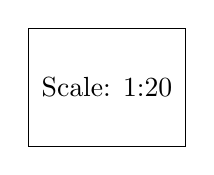
\begin{tikzpicture}[scale=0.5]
\draw (0,0) rectangle (4,3);
\node at (2,1.5) {Scale: 1:20};
\end{tikzpicture}
\end{center}

\item \ealpara{James robi \ealkeytr{skalowany} model samochodu. Rzeczywisty samochód ma 4.2 metra długości, a jego model ma 28 cm długości. Jakie \ealkeytr{skalowanie} stosuje? Wyraź odpowiedź jako \ealkeytr{stosunek} w \ealkeytr{najprostszej postaci}.}{James is making a \ealkey{scale} model of a car. The actual car is 4.2 meters long, and his model is 28 cm long. What \ealkey{scale} is he using? Express your answer as a \ealkey{ratio} in \ealkey{simplest form}.}

\item \ealpara{Mapa ma \ealkeytr{skalowanie}, w którym 4 cm odpowiada 5 km. Dwa miasta są oddalone na mapie o 15.2 cm.}{A map has a \ealkey{scale} where 4 cm represents 5 km. Two cities appear 15.2 cm apart on the map.}
\begin{enumerate}
    \item \ealpara{Jaka jest rzeczywista odległość między miastami?}{What is the actual distance between the cities?}
    \item \ealpara{Jakie jest \ealkeytr{skalowanie} mapy wyrażone jako \ealkeytr{stosunek}?}{What is the map \ealkey{scale} expressed as a \ealkey{ratio}?}
    \item \ealpara{Jeśli inna mapa używa \ealkeytr{skalowania} 1:125,000, która mapa pokazuje więcej szczegółów (większe \ealkeytr{skalowanie})?}{If another map uses \ealkey{scale} 1:125,000, which map shows more detail (larger \ealkey{scale})?}
\end{enumerate}

\item \ealpara{Plan podłogi małego pokoju ma 6 metrów długości i 4.5 metra szerokości. Korzystając z kratkowanego tła poniżej, stwórz \ealkeytr{skalowany} rysunek tego pokoju. Użyj \ealkeytr{skalowania} \newline 1 cm : 1 m. Wyraźnie zaznacz wymiary na rysunku.}{The floor plan of a small room is 6 meters long and 4.5 meters wide. Using the squared background below, create a \ealkey{scale} drawing of this room. Use a \ealkey{scale} of \newline 1 cm : 1 m. Clearly label the dimensions on your drawing.}
\begin{center}

\begin{tikzpicture}
\draw[step=1cm, gray, very thin] (0,0) grid (10,7);
\end{tikzpicture}
\end{center}

\end{enumerate}

\newpage{}

\section*{\ealkey{Rates} of Change}

\begin{enumerate}
    \item \ealpara{Rowerzysta pokonuje \SI{45}{\kilo\metre} w 1 godzinę i 30 minut. Oblicz jej \ealkeytr{średnią} \ealkeytr{prędkość} w \si{\kilo\metre\per\hour}.}{A cyclist travels \SI{45}{\kilo\metre} in 1 hour and 30 minutes. Calculate her \ealkey{average} \ealkey{speed} in \si{\kilo\metre\per\hour}.}

    \item \ealpara{Woda płynie z kranu ze \ealkeytr{stałą} \ealkeytr{wielkością ilorazową}. Napełnienie \SI{12}{\litre} konewki zajmuje 3 minuty. Przy tej \ealkeytr{wielkości ilorazowej}, ile czasu zajęłoby napełnienie \SI{90}{\litre} zbiornika na wodę?}{Water flows from a tap at a \ealkey{constant} \ealkey{rate}. It takes 3 minutes to fill a \SI{12}{\litre} watering can. At this \ealkey{rate}, how long would it take to fill a \SI{90}{\litre} water butt?}

    \item \ealpara{Pociąg wyjeżdża z Londynu o 10:15 i przyjeżdża do Yorku, oddalonego o \SI{320}{\kilo\metre}, o 14:45. Zatrzymuje się na 10 minut na stacji w połowie podróży. Oblicz \ealkeytr{średnią} \ealkeytr{prędkość} pociągu dla całej podróży, \textbf{włączając} postój. A co z \ealkeytr{średnią} \ealkeytr{prędkością}, gdy pociąg był w ruchu?}{A train leaves London at 10:15 and arrives in York, \SI{320}{\kilo\metre} away, at 14:45. It stops for 10 minutes at a station halfway through the journey. Calculate the train's \ealkey{average} \ealkey{speed} for the whole journey, \textbf{including} the stop. What about the \ealkey{average} \ealkey{speed} when the train was in motion?}

    \item \ealpara{W zlewce zachodzi reakcja chemiczna. Na początku zlewka zawiera \SI{400}{\gram} substancji A. Reakcja zużywa A z \ealkeytr{wielkością ilorazową} 4 gramy na minutę, ile substancji A pozostaje w zlewce po 4 minutach?}{A chemical reaction happens in a beaker. At the start, the beaker contains \SI{400}{\gram} of chemical A. The reaction uses up A at a \ealkey{rate} of 4 grams per minute, how much chemical A is left in the beaker after 4 minutes?}

    \item \ealpara{Sarah jedzie autostradą. Jedzie przez \SI{30}{\minute} ze \ealkeytr{średnią} \ealkeytr{prędkością} \SI{60}{\text{miles}\per\hour}. Następnie zatrzymuje się na stacji serwisowej na 15 minut. Kończy podróż, jadąc kolejne \SI{45}{\minute} ze \ealkeytr{średnią} \ealkeytr{prędkością} \SI{50}{\text{miles}\per\hour}.}{Sarah is driving on a motorway. She drives for \SI{30}{\minute} at an \ealkey{average} \ealkey{speed} of \SI{60}{\text{miles}\per\hour}. She then stops at a service station for 15 minutes. She completes her journey by driving for another \SI{45}{\minute} at an \ealkey{average} \ealkey{speed} of \SI{50}{\text{miles}\per\hour}.}
    \begin{enumerate}
        \item \ealpara{Oblicz całkowitą odległość jej podróży.}{Calculate the total distance of her journey.}
        \item \ealpara{Oblicz jej \ealkeytr{średnią} \ealkeytr{prędkość} dla \textbf{całej podróży}, włączając postój.}{Calculate her \ealkey{average} \ealkey{speed} for the \textbf{whole journey}, including the stop.}
    \end{enumerate}

\end{enumerate}

\vspace{3cm}

\section*{Problem Solving With \ealkey{Ratios}}
\begin{enumerate}

    \item \ealpara{\ealkeytr{Stosunek} czerwonych do niebieskich kulek w torbie wynosi $3:5$. Jeśli dodano 8 czerwonych kulek, \ealkeytr{stosunek} staje się $5:7$. Ile jest niebieskich kulek?}{The \ealkey{ratio} of red to blue marbles in a bag is $3:5$. If 8 red marbles are added, the \ealkey{ratio} becomes $5:7$. How many blue marbles are there?}

    \item \ealpara{\ealkeytr{Stosunek} jabłek, bananów i pomarańczy w koszyku z owocami wynosi $2:5:3$. Po dodaniu 4 jabłek i 2 bananów nowy \ealkeytr{stosunek} jabłek do bananów do pomarańczy wynosi $4:6:3$ Ile pomarańczy jest w koszyku?}{The \ealkey{ratio} of apples, bananas, and oranges in a fruit basket is $2:5:3$. After 4 apples and 2 bananas are added, the new \ealkey{ratio} of apples to bananas to oranges is $4:6:3$ How many oranges are in the basket?}

    \item \ealpara{\ealkeytr{Stosunek} cukru do mąki w przepisie wynosi $2:9$. \ealkeytr{Stosunek} mąki do masła wynosi $3:1$. Znajdź \ealkeytr{stosunek} cukru do mąki do masła.}{The \ealkey{ratio} of sugar to flour in a recipe is $2:9$. The \ealkey{ratio} of flour to butter is $3:1$. Find the \ealkey{ratio} of sugar to flour to butter.}

    \item \ealpara{Kwota pieniędzy jest dzielona między Alexa, Bena i Chloe w \ealkeytr{stosunku} $3:4:5$. Jeśli Ben otrzymuje £40 więcej niż Alex, znajdź całkowitą kwotę pieniędzy.}{A sum of money is divided between Alex, Ben, and Chloe in the \ealkey{ratio} $3:4:5$. If Ben receives £40 more than Alex, find the total sum of money.}

    \item \ealpara{Punkty $A$, $B$ i $C$ leżą na prostej. \ealkeytr{Stosunek} $AB$ do $BC$ wynosi $3:2$. Jeśli $AB = 12$ cm, znajdź długość $AC$.}{The points $A$, $B$, and $C$ lie on a straight line. The \ealkey{ratio} of $AB$ to $BC$ is $3:2$. If $AB = 12$ cm, find the length of $AC$.}

    \item \ealpara{Torba zawiera żetony w trzech kolorach: czerwonym, żółtym i niebieskim. \ealkeytr{Stosunek} czerwonych do żółtych wynosi $3:4$. \ealkeytr{Stosunek} żółtych do niebieskich wynosi $5:6$. Jaki \ealkeytr{ułamek} żetonów jest niebieski?}{A bag contains counters in three colours: red, yellow, and blue. The \ealkey{ratio} of red to yellow is $3:4$. The \ealkey{ratio} of yellow to blue is $5:6$. What \ealkey{fraction} of the counters are blue?}

    \item \ealpara{\ealkeytr{Stosunek} czerwonych do niebieskich kulek w torbie wynosi $2:3$. Po dodaniu $36$ czerwonych kulek i $29$ niebieskich kulek \ealkeytr{stosunek} staje się $4:5$. Ile niebieskich kulek było początkowo w torbie?}{The \ealkey{ratio} of red to blue marbles in a bag is $2:3$. After $36$ red marbles, and $29$ blue marbles are added the \ealkey{ratio} becomes $4:5$. How many blue marbles were in the bag initially?}

\end{enumerate}

\end{document}